% Lines that start with a % are comments and are not included when the LaTeX file is converted to a pdf

% Set up the document class - this can be changed if a different format is required 
\documentclass[11pt,a4paper,twoside]{article}

% Include packages that contain additional features, for example including special mathematical characters and images in your document
\usepackage{amssymb,amsmath,graphicx}
\usepackage[T1]{fontenc} 
\usepackage[utf8]{inputenc}   % here are our umlauts...
\usepackage{graphicx} % ...and our graphics
\usepackage{listings}
\usepackage{bold-extra}
\usepackage[plainpages=false, pdfpagelabels, colorlinks=true, breaklinks=true, linkcolor=black, menucolor=black, urlcolor=black, citecolor=black]{hyperref}
\usepackage[font=sf, labelfont={sf,bf}, margin=1cm]{caption}
\usepackage[b]{esvect}
% Long equations
\usepackage{breqn} 
%include pdfs
\usepackage{pdfpages}
\usepackage{hyperref}
\usepackage{epstopdf}
%\usepackage{fullpage}
\usepackage{placeins}
\usepackage{pdfpages}


% The beginning of the document...
\begin{document}
\renewcommand\thesubsection{\alph{subsection})}

% configure standard code listings:
\lstset {
language = bash,
	breaklines = true,
	breakatwhitespace = true
}

% Please change the following accordingly...
\centerline{\LARGE \textbf{Artificial Intelligence - Exercise Sheet 5}}\vspace{0.5em}
\centerline{\large by Lucas-Raphael Müller}\vspace{2em}


\textit{I had the impression that this weeks exercise was quite much and would have been better split over two weeks.}
\section{Tic Tac Toe}
\subsection{General Design}
Suitable utility values should agree with our evaluation function. 
Therefore $u \in \{-1, 0, 1\}$ for a lost, draw or won scenario are reasonable choices.
The tree can not get deeper than the number of fields in the tic tac toe case.
The depth is therefore 9 (or including the empty board 10).
If one does not stop going deeper even when the game is already won, the number of nodes can be calculated by
\begin{equation}
	n < \sum\limits_{i = 1}^9 \frac{9!}{i!}.
\end{equation}
It is not easy (if not not possible) to give a closed form equation excluding the nodes when the game is already won, therefore it's an upper limit. 

\subsection{Implementation and Testing}
I designed a few test cases to ensure correctly working minimax algorithm and board behaviour.
All tesets \textbf{passed}.
They can be found in 4 \ref{sub:testing} and can be executed via \textit{python -m pytest test_board.py} locally or automatically as below.
Testing has been done on \textit{Travis CI}.\footnote{\url{https://travis-ci.org/Haydnspass/artificial_intelligence}}

\section{Pruning}
\textit{Correction:} It's sufficient to know 1-3 and 5 since the expected value of the left hand side can not be achieved with any number of 6-8, therefore 4 is also not needed.
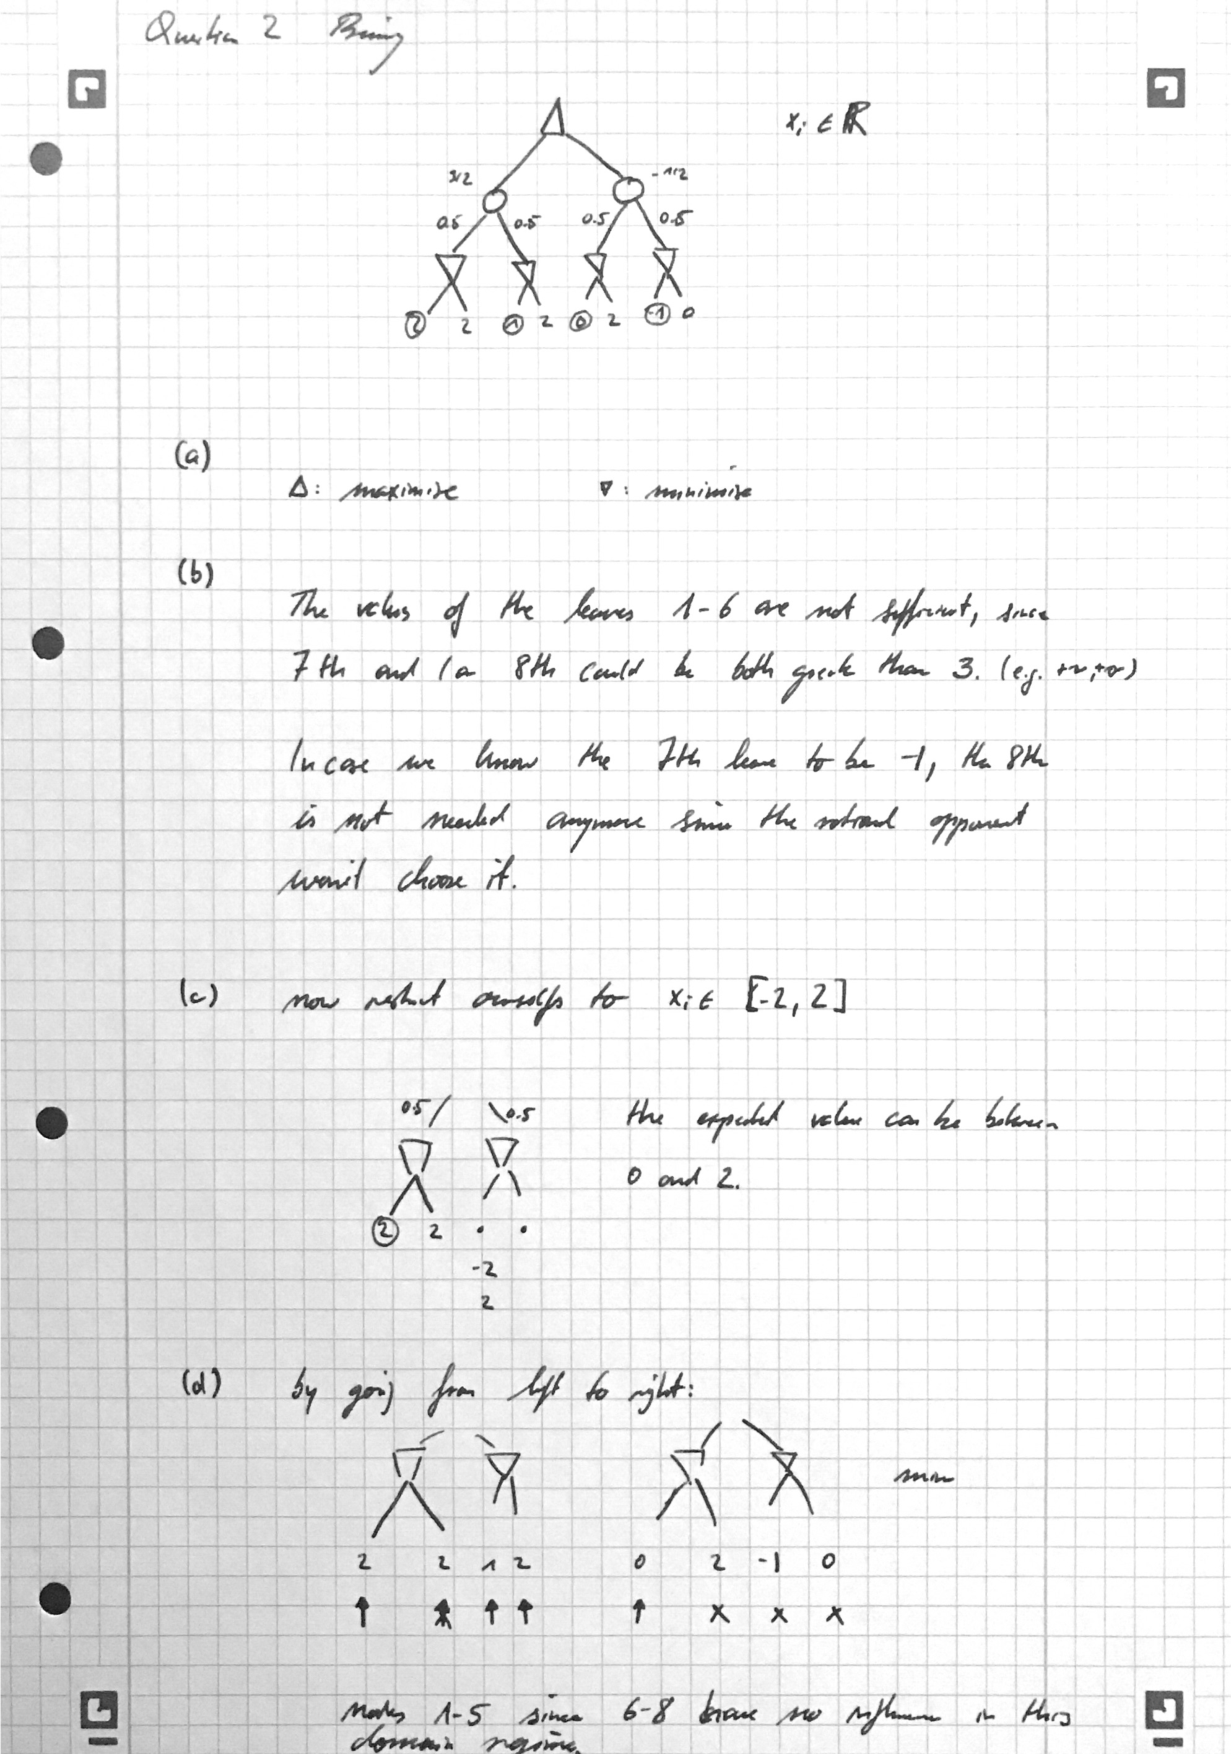
\includepdf[pages={1}]{figures/pruning.pdf}

\section{Four Dices Straight}
\subsection*{General Approach}
In principle we can form 4 categories of moves, i.e. the different number of dices we roll again. There are
\begin{itemize}
	\item 4 possibilities to roll 1 dice,
	\item 6 to roll 2,
	\item 4 to roll 3,
	\item 1 to roll all 4.
\end{itemize}
The total number of outcomes are $6^{n_{redrawn}}$ where many are equal, because one does not care about the order.
This could be similiarily implemented as tic tac toe but accounting for a chance game.


\FloatBarrier

\newpage
\section{Appendix: Python Source Code}
\label{sec:app}

\subsection{Testing minimax}
\label{sub:testing}
\lstinputlisting[language=Python]{test_board.py}

\subsection{Code}
\lstinputlisting[language=Python]{tictactoe.py}

\end{document}
